% Fig. 1 kaynagi: sistem mimarisi. Derleme:
%   pdflatex system_architecture.tex  ->  ../system_architecture.pdf olarak kopyala
\documentclass[tikz,border=2pt]{standalone}
\usepackage[T1]{fontenc}
\usepackage[scaled=0.92]{helvet}
\renewcommand{\familydefault}{\sfdefault}
\usetikzlibrary{positioning,fit,arrows.meta,calc,backgrounds}

\definecolor{memfill}{HTML}{FFF4D6}\definecolor{memline}{HTML}{B8860B}
\definecolor{dpfill}{HTML}{E3F2E3}\definecolor{dpline}{HTML}{2E7D32}
\definecolor{axifill}{HTML}{E1ECF8}\definecolor{axiline}{HTML}{1F5FA8}
\definecolor{psfill}{HTML}{ECECEF}\definecolor{psline}{HTML}{55555F}

\tikzset{
  blk/.style={draw, rounded corners=2pt, line width=0.6pt, align=center,
              inner sep=3pt, font=\footnotesize},
  mem/.style={blk, fill=memfill, draw=memline},
  dp/.style={blk, fill=dpfill, draw=dpline},
  axi/.style={blk, fill=axifill, draw=axiline},
  ps/.style={blk, fill=psfill, draw=psline},
  grp/.style={draw=black!45, dashed, rounded corners=3pt, inner sep=5pt},
  grplbl/.style={font=\scriptsize\ttfamily, text=black!60, anchor=south west, inner sep=1pt},
  dat/.style={-{Latex[length=4pt]}, line width=0.6pt},
  bid/.style={{Latex[length=4pt]}-{Latex[length=4pt]}, line width=0.6pt},
  ctl/.style={-{Latex[length=4pt]}, line width=0.6pt, dashed},
  lbl/.style={font=\scriptsize, fill=white, inner sep=1pt},
}

\begin{document}
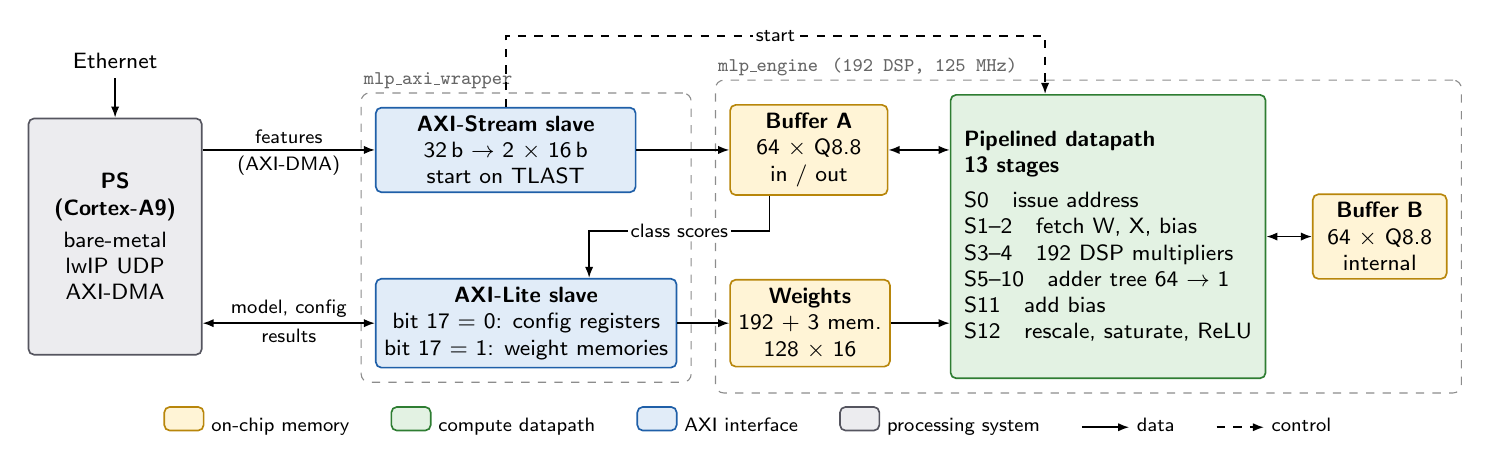
\begin{tikzpicture}

% satirlar: ust = veri yolu, alt = yapilandirma yolu
\def\yt{11mm}\def\yb{-11mm}

\node[ps, minimum width=22mm, minimum height=30mm] (ps) at (0,0)
  {\textbf{PS}\\\textbf{(Cortex-A9)}\\[2pt]bare-metal\\lwIP UDP\\AXI-DMA};
\node[above=5mm of ps, font=\footnotesize] (eth) {Ethernet};
\draw[dat] (eth) -- (ps);

\node[axi, minimum width=33mm, anchor=west] (axis) at (33mm,\yt)
  {\textbf{AXI-Stream slave}\\32\,b $\to$ 2 $\times$ 16\,b\\start on TLAST};
\node[axi, minimum width=33mm, anchor=west] (axil) at (33mm,\yb)
  {\textbf{AXI-Lite slave}\\bit 17 = 0: config registers\\bit 17 = 1: weight memories};

\node[mem, minimum width=20mm, anchor=west] (bufa) at (78mm,\yt)
  {\textbf{Buffer A}\\64 $\times$ Q8.8\\in / out};
\node[mem, minimum width=20mm, anchor=west] (wmem) at (78mm,\yb)
  {\textbf{Weights}\\192 + 3 mem.\\128 $\times$ 16};

\node[dp, minimum width=40mm, minimum height=36mm, anchor=west, align=left] (core) at (106mm,0)
  {\textbf{Pipelined datapath}\\\textbf{13 stages}\\[3pt]
   S0\quad issue address\\
   S1--2\quad fetch W, X, bias\\
   S3--4\quad 192 DSP multipliers\\
   S5--10\quad adder tree 64 $\to$ 1\\
   S11\quad add bias\\
   S12\quad rescale, saturate, ReLU};

\node[mem, minimum width=17mm, anchor=west] (bufb) at (152mm,0)
  {\textbf{Buffer B}\\64 $\times$ Q8.8\\internal};

\begin{scope}[on background layer]
  \node[grp, fit=(axis)(axil)] (gw) {};
  \node[grp, fit=(bufa)(wmem)(core)(bufb)] (ge) {};
\end{scope}
\node[grplbl] at (gw.north west) {mlp\_axi\_wrapper};
\node[grplbl] at (ge.north west) {mlp\_engine \,(192 DSP, 125 MHz)};

% veri yolu
\draw[dat] (ps.east |- axis) -- node[lbl, above=1pt] {features} node[lbl, below=1pt] {(AXI-DMA)} (axis.west);
\draw[dat] (axis.east) -- (bufa.west);
\draw[bid] (bufa.east) -- (bufa.east -| core.west);
\draw[bid] (core.east) -- (bufb.west);
\draw[ctl] (axis.north) -- ++(0,9mm) -| node[lbl, pos=0.25] {start} ([xshift=-8mm]core.north);
% yapilandirma yolu
\draw[bid] (ps.east |- axil) -- node[lbl, above=1pt] {model, config} node[lbl, below=1pt] {results} (axil.west);
\draw[dat] (axil.east) -- (wmem.west);
\draw[dat] (wmem.east) -- (wmem.east -| core.west);
\draw[dat] ([xshift=-5mm]bufa.south) -- ++(0,-4.5mm) -| node[lbl, pos=0.25] {class scores} ([xshift=8mm]axil.north);

% lejant
\node[anchor=north, font=\scriptsize] at ($(ps.south)!0.5!(bufb.south) + (0,-10mm)$) {%
  \tikz\node[mem, minimum width=5mm, minimum height=3mm]{};\ on-chip memory\qquad
  \tikz\node[dp, minimum width=5mm, minimum height=3mm]{};\ compute datapath\qquad
  \tikz\node[axi, minimum width=5mm, minimum height=3mm]{};\ AXI interface\qquad
  \tikz\node[ps, minimum width=5mm, minimum height=3mm]{};\ processing system\qquad
  \tikz\draw[dat](0,0)--(6mm,0);\ data\qquad
  \tikz\draw[ctl](0,0)--(6mm,0);\ control};
\end{tikzpicture}
\end{document}
